\documentclass[11pt]{amsart}
\usepackage[margin=1in, marginparwidth=0.8in]{geometry}
\usepackage{xcolor}
\usepackage[colorlinks,linkcolor=black!50!red,citecolor=blue,pdfpagemode=None]{hyperref}
\usepackage[capitalise]{cleveref}
\usepackage{graphicx}

% shorthands 
\newcommand{\cA}{\mathcal{A}}
\newcommand{\bC}{\mathbb{C}}
\newcommand{\cAb}{\mathcal{A}_\bullet}
\newcommand{\Supp}{\operatorname{Supp}}
\newcommand{\ZZ}{\mathbb{Z}}
\newcommand{\bg}{\mathbf{g}}
\newcommand{\bc}{\mathbf{c}}
\newcommand{\bb}{\mathbf{b}}
\newcommand{\id}{\mathrm{id}}

% ambients and numbering
\newtheorem{theorem}{Theorem}[section]
\newtheorem{conjecture}[theorem]{Conjecture}
\newtheorem{corollary}[theorem]{Corollary}
\newtheorem{lemma}[theorem]{Lemma}
\newtheorem{proposition}[theorem]{Proposition}
\newtheorem{example}[theorem]{Example}
\theoremstyle{definition}
\newtheorem{remark}[theorem]{Remark}
\newtheorem{definition}[theorem]{Definition}
\numberwithin{equation}{section}
\numberwithin{figure}{section}

\begin{document}
\title[Exchange relations for finite type cluster algebras]{Exchange relations for finite type cluster algebras with acyclic initial seed and principal coefficients}

\author[Stella]{Salvatore Stella}
\address[Salvatore Stella]{IN$d$AM - Marie Curie Actions fellow, Universit\`a ``La Sapienza'', Roma, Italy.}
\email{stella@mat.uniroma1.it}

\author[tumarkin]{Pavel Tumarkin}
\address[Pavel Tumarkin]{Department of Mathematical Sciences, Durham University, UK}
\email{pavel.tumarkin@durham.ac.uk}

\begin{abstract}
We give an explicit description of all the exchange relations in any finite type cluster algebra with acyclic initial seed and principal coefficients.
\end{abstract}

\maketitle

\section{Introduction and main results}
  A cluster algebra, as defined by Fomin and Zelevinsky in~\cite{FZ02}, is a commutative ring with a distinguished set of generators called \emph{cluster variables}. 
  Cluster variables are grouped into overlapping collections of the same cardinality (\emph{clusters}) connected by local transition rules called \emph{mutations}.
  To each mutation corresponds an \emph{exchange relation}: a dependency relation among the cluster variables of two adjacent clusters.
  In~\cite{FZ03}, Fomin and Zelevinsky showed that cluster algebras of \emph{finite type}, i.e. those containing only a finite number of cluster variables, are classified by finite type Cartan matrices.

  Given two cluster variables in a cluster algebra, deciding whether they belong to the same cluster or if they can be obtained from one another by a single mutation is, in general, a hard problem to address.
  In some special situations though, when suitable combinatorial models exist, such questions become much easier to decide.
  This is the case, for example, of cluster algebras of finite type with an acyclic initial seed where the answer is given using the \emph{compatibility degree} of the corresponding \emph{$\bg$-vectors}.
  
  Knowing that two cluster variables are exchangeable naturally arises the problem of producing the exchange relation they satisfy.
  There are two partial answers to this question when the algebra is of finite type and has an acyclic initial seed. 
  In \cite{YZ08}, using some determinantal identities on the associated Lie group, the authors were able to give explicit formulas for all the \emph{primitive} exchange relations (i.e. those in which cluster variables only appear in one of the two monomials of the right hand side). 
  Their recipe works for principal coefficients and hence, via separation of additions, for any choice of coefficients.

  In \cite{Ste13} the first author gave a uniform formula for all the exchange relations, albeit only in the coefficient-free case.
  The main goal of the current paper is to improve on this result to deal with principal coefficients as well. 
  Namely, given any two exchangeable cluster variables in a finite type cluster algebra with acyclic initial seed and principal coefficients, we give an explicit formula for computing their exchange relation.
  This exchange relation has also a geometric interpretation in terms of roots and weights of the corresponding root system.

 
  In order to make this more precise, we need to recall few notions and results from \cite{Ste13,YZ08}.

  Let $A=(a_{ij})$ be any finite type Cartan matrix; we denote by $\Gamma$ its Dynkin diagram and by $W=\langle s_1,\dots,s_n\rangle$ the associated Weyl group and simple reflections.
  To each \emph{Coxeter element} $c=s_{i_1}\cdots s_{i_n}$ in $W$ we can associate a skew-symmetrizable integer matrix $B_c=(b_{ij})_{i,j\in[1,n]}$ by setting
  \[
    b_{ij}=
    \begin{cases}
      -a_{ij} & \text{if } i\prec_c j  \\
      a_{ij}  & \text{if } j\prec_c i  \\
      0       & \text{otherwise}
    \end{cases}
  \]
  where we write $i\prec_c j$ if and only if $s_i$ precedes $s_j$ in all reduced expressions of $c$.
  As $c$ varies, we get all possible \emph{acyclic} exchange matrices of the same cluster algebra.
  We will denote by $\cA_\bullet(c)$ the cluster algebra with initial exchange matrix $B_c$ and  \emph{principal coefficients} at the initial seed.

  The algebra $\cA_\bullet(c)$ is $\ZZ^n$-graded; its cluster variables and cluster monomials are homogeneous elements and their \emph{$\bg$-vector} is their homogeneous degree (see~\cite[Section~6]{FZ07}).
  Let $\omega_i$ be the i-th \emph{fundamental weight} in the \emph{weight lattice} $P$ of $\Gamma$; we will routinely interpret $\bg$-vectors as weights by writing them in the basis of fundamental weights.

  Let $w_0$ be the longest element of $W$ and denote by $h(i;c)$ the minimum positive integer such that 
  \[
    c^{h(i;c)}\omega_i = w_0\omega_i
  \]
  (it is a finite number \cite[Proposition 1.3]{YZ08}).
  \begin{theorem}[{\cite[Theorem 1.4]{YZ08}}]
    The cluster variables of $\cA_\bullet(c)$ are naturally in bijection with the elements of the set
    \[
      \Pi(c)
      :=
      \left\{
        c^m\omega_i \, :\, i\in[1,n] \, , \, 0\leq m \leq h(i;c) 
      \right\}.
    \]
    To the cluster variable $x_\lambda$ it corresponds its $\bg$-vector $\lambda\in\Pi(c)$.
  \end{theorem}
  This correspondence extends to a bijection between points of $P$ and \emph{cluster monomials} of $\cA_\bullet(c)$ (cf. \cite[Theorem 1.2]{Ste13}); for $\lambda\in P$ we will denote by $x_\lambda$ the cluster monomial whose $\bg$-vector is $\lambda$.

  The set $\Pi(c)$ is naturally endowed with a permutation $\tau_c$ defined by
  \[
    \tau_c (\lambda) 
    :=
    \begin{cases}
      \omega_i  & \text{if $\lambda = -\omega_i$} \\
      c\lambda  & \text{otherwise}
    \end{cases}
  \]
  which extends to a piecewise linear map on the whole of $P$ that is ``compatible'' with the cluster structure of $\cA_\bullet(c)$.
  This is a combinatorial shadow of a notable automorphism of the coefficient-free counterpart of $\cA_\bullet(c)$ sending the cluster variable $x_\lambda$ to $x_{\tau_c(\lambda)}$. 

  Let $Q$ be the \emph{root lattice} of $\Gamma$ with simple roots $\alpha_i$; as for $P$, we will routinely think of elements in $Q$ as integer vectors using the basis of simple roots.
  \begin{definition}
    The \emph{compatibility degree} $(\cdot||\cdot)_c$ is the unique $\tau_c$-invariant function on pairs of elements of $\Pi(c)$ defined by the initial conditions
    \[
      (\omega_i||\lambda)_c
      :=
      \left[ (c^{-1}-\id)\lambda ; \alpha_i\right]_+
    \]
    where, for $v$ in $Q$, $[v;\alpha_i]$ denotes the $i$-th coefficient of $v$  and $[m]_+$ is a shorthand for $\max\{m, 0\}$ (cf. \cite[Proposition 5.1]{YZ08}).
  \end{definition}
  The name comes from the following important property, consequence of the polytopal realization of the cluster fan of $\cA_\bullet(c)$ (\cite{CFZ02,Ste13}).
  \begin{proposition}
    Two weights $\lambda$ and $\mu$ from $\Pi(c)$ are
    \begin{itemize}
      \item
        \emph{compatible} (i.e. there is a cluster of $\cA_\bullet(c)$ containing both $x_\lambda$ and $x_\mu$) if and only if
        \[
          (\lambda||\mu)_c = 0
          \quad \quad
          \text{(equivalently $(\mu||\lambda)_c=0$)}
        \]

      \item
        \emph{exchangeable} (i.e. there are two clusters of $\cA_\bullet(c)$ that can be obtained from one-another by swapping $x_\lambda$ for $x_\mu$) if and only if
        \[
          (\lambda||\mu)_c = 1 = (\mu||\lambda)_c
        \]
    \end{itemize}
  \end{proposition}

  Our starting point is the following restatement of \cite[Proposition 5.1]{Ste13}. 
  \begin{proposition}
    Suppose $\lambda$ and $\mu$ are exchangeable weights in $\Pi(c)$. 
    Then the set
    \[
      \left\{
        \tau_c^{-m}\left(\tau_c^m(\lambda)+\tau_c^m(\mu)\right)
      \right\}_{m\in\ZZ}
    \]
    consists precisely of two weights. 
    One of them is $\lambda+\mu$; denote the other by $\lambda\uplus_c\mu$.
  \end{proposition}

  Let $y_1,\dots,y_n$ be the generators of the coefficient semifield of $\cA_\bullet(c)$ and denote by $y^\alpha$ the product $\prod_{i=1}^n y_i^{[\alpha;\alpha_i]}$.

  \begin{theorem}
    \label{thm:main}
    Suppose $\lambda$ and $\mu$ are exchangeable weights in $\Pi(c)$. 
    Then there exists a unique  positive root  $\alpha$ in the root system of $\Gamma$ such that
    \begin{equation}
      \label{eq:system}
      -B_c\alpha = \lambda+\mu-\lambda\uplus_c\mu
    \end{equation}
    and
    \begin{equation}
      \label{eq:dual}
      \langle\lambda,\alpha^\vee\rangle 
      \langle\mu,\alpha^\vee\rangle 
      = -1
    \end{equation}
    (here $\alpha^\vee$ denotes the \emph{coroot} corresponding to $\alpha$ while $\langle\cdot\,,\cdot\rangle$ is the pairing of dual vector spaces).
    Moreover the cluster variables $x_\lambda$ and $x_\mu$ of $\cA_\bullet(c)$ satisfy the exchange relation
    \begin{equation}
      \label{eq:exrel}
      x_\lambda x_\mu = x_{\lambda+\mu} + y^\alpha x_{\lambda\uplus_c\mu}.
    \end{equation}
   \end{theorem}

  Note that the shape of \cref{eq:exrel} follows immediately from the coefficient-free case \cite[Proposition 5.2]{Ste13} together with the observations that $\bc$-vectors are roots in the root system of $\Gamma$ (cf. \cite{NS14})  and that the exchange relations in $\cA_\bullet(c)$ are homogeneous.
  The real content of our theorem are therefore the explicit conditions~\cref{eq:system} and~\cref{eq:dual} that determine $\alpha$. 
  They are clearly both necessary.

  Indeed, \cref{eq:system} is just a restatement of the fact that the exchange relations in $\cA_\bullet(c)$ are homogeneous and that the degree of $y_i$ is $-\bb_i$ (the negative of the i-th column of $B_c$).
  \cref{eq:dual}, instead, follows immediately from \cite[Eq. (1.11)]{NZ12} once we interpret $\bg$-vectors as weights and $\bc$-vectors as roots together with the observation that, when mutating in direction $k$, the $k$-th $\bc$-vector changes into its negative.
  
  On the other hand, \cref{eq:system} is not, in principle, sufficient on its own because $B_c$ is, in general, not invertible.
  Nonetheless, thanks to the fact that we are dealing with positive roots, we will see that it is still enough in every case except in type $D_n$.
  
  \begin{remark}
    \label{geom}
    \cref{eq:system} has the following geometric interpretation.
    Associating the $\bg$-vectors with weights, one can observe that every cluster corresponds to a cone with facets being mirrors of reflections of the associated Weyl group (see \cref{fig:exchange_relation}).
    If two clusters are neighbors in the exchange graph (i.e. they differ only by two exchangeable cluster variables $x_\lambda$ and $x_\mu$), then the corresponding cones share a facet, and this facet is precisely the mirror of the reflection in the root $\alpha$ from \cref{eq:system}.
   \begin{figure}[h]
      \begin{center}
        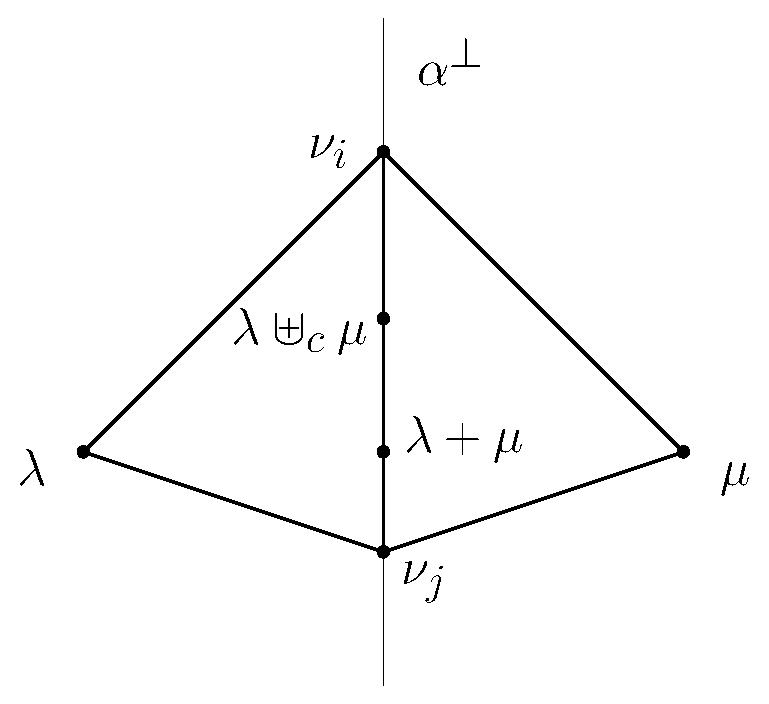
\includegraphics[scale=0.4]{cones-section.eps}
      \end{center}
      \caption{Exchange relation: $x_\lambda$ and $x_\mu$ are exchangeable cluster variables, $\alpha$ is the required root.}
      \label{fig:exchange_relation}
    \end{figure}
\end{remark} 
 
\subsection*{Acknowledgments}
  This paper was completed during a visit to Durham University; the first author would like to thank both Grey College and the Department of Mathematics for the hospitality received.
  We are also grateful to Anna Felikson for many fruitful discussions, and to Nathan Reading for his help with some early attempts at \cref{thm:main} and for his comments on a preliminary version of this paper.
 
\section{Proof of \cref{thm:main}}
\label{proof}
  Recall the notation for $\Gamma$, $c$ and $B_c$ from the previous section. 
  Without loss of generality we consider only Dynkin diagrams that are connected.
  Further, we assume that the nodes of $\Gamma$ are labeled according to the standard conventions as, for example, in \cite[Table Fin.]{Kac90}.

  We begin our analysis with a well known consideration on the rank of $B_c$.
  \begin{lemma}
    \label{lem:dimensions}
    If the type of $\Gamma$ is not $D_n$, then the kernel of $B_c$ has dimension $0$ if $n$ is even and $1$ if $n$ is odd.
    If the type of $\Gamma$ is $D_n$, then the kernel of $B_c$ has dimension $2$ if $n$ is even and $1$ if $n$ is odd.
  \end{lemma}
  \begin{proof}
    The rank of $B_c$ is invariant under mutations so it suffices to establish the property for a single choice of $c$. 
    Let then $c=s_1\cdots s_n$ so that $B_c$ has positive entries above the diagonal.
    Exceptional types could be dealt uniformly in the argument at the expense of introducing heavier notation. 
    We prefer to check the lemma by direct inspection in those cases.

    Assume at first that the type of $\Gamma$ is not $D_n$.
    When $n$ is even, the matrix $B_c$ is invertible. 
    Indeed, expanding by the first column and then by the first row, we get:
    \[
      \det(B_c)=-\det(B_c')
    \]
    where $B_c'$ is a $(n-2)\times(n-2)$ matrix in the same infinite class of $B_c$. 
    The result follows then immediately by induction because all $2\times2$ skew-symmetrizable non-zero matrices are invertible.
    The same argument, with $n=1$ as base of the induction, shows that when $n$ is odd $\det(B_c)=0$.
    Combining the two assertions we get that, for odd $n$, the dimension of the kernel of $B_c$ is $1$.

    To get the result in type $D_n$ it is enough to observe that the last two rows (and columns) of $B_c$ are identical. 
    We deduce therefore the required property from type $A_{n-1}$.
  \end{proof}

  This establishes \cref{thm:main} whenever $n$ is even and the type of $\Gamma$ is not $D_n$.
  In particular the result holds for all the exceptional types apart from type $E_7$; in order to simplify the remaining analysis we check this exceptional case by direct inspection.
  From now on we assume that $\Gamma$ is not of exceptional type.

  \begin{remark}
    \label{rk:induction}
    A careful reader may observe that \cref{lem:dimensions} could be used to establish \cref{thm:main} directly in all finite types with the exception of $D_n$. 
    Indeed it would be enough to extend any $(2k+1) \times (2k+1)$ exchange matrix to a $(2k+2) \times (2k+2)$ exchange matrix of the same type and deduce the required property from the resulting algebra embedding.
    Instead, we prefer to give a more explicit argument that will simplify the analysis in type $D_n$ as well.
  \end{remark}

  To deal with the remaining infinite families we compute explicit generators for the kernel of $B_c$. 
  Our argument will hinge upon an explicit description of the possible differences of positive roots; unfortunately in small rank non-generic situations may arise.
  We therefore verify \cref{thm:main} by direct inspection in types $A_3$, $B_3$, $C_3$, and $D_4$.

  \begin{definition}
    The \emph{support} of a vector $v$ is the full subdiagram of $\Gamma$ induced by the nodes corresponding to the non-zero coordinates of $v$ when written in the basis of simple roots.
  \end{definition}

  \begin{lemma}
    Let $\Gamma$ be of type $A_n$, $B_n$, or $C_n$ with $n=2k+1$.
    Then the support of the vector spanning the kernel of $B_c$ has exactly $k+1$ connected components. 
  \end{lemma} 
  \begin{proof}
    By \cref{lem:dimensions} there is a unique (up to a scalar) non-zero vector $v$ such that $B_cv=0$.
    Since the only non-zero entries in $B_c$ are located in the two diagonals adjacent to the main diagonal, $v$ is a linear combination of the $\alpha_i$ with odd $i$.
    Moreover, since $\Gamma$ is connected, all the entries of these two diagonals are non-zero so that all such $\alpha_i$ appear with non-zero coefficient and the claim follows.
    
    More explicitly, for $i>2$ set 
    \[
      \varepsilon_i :=
      \begin{cases}
        1 & \text{if $i-2\prec_c i-1 \prec_c i$ or $i\prec_c i-1 \prec_c i-2$}\\
        -1 & \text{otherwise.}
      \end{cases}
    \]
    It is straightforward to verify that the kernel of $B_c$ is spanned by the vector $v$ defined by
    \begin{equation}
      \label{eq:vector}
      v := 
      \alpha_1 + \sum_{\substack{i\ \mathrm{odd}\\ 3\le\, i\,\leq n}} \frac{\varepsilon_i}{a_{i-1,i}} \alpha_i.
    \end{equation}
  \end{proof}
  
  \begin{lemma}
    \label{lem:ker_Dn_even}
    Let $\Gamma$ be of type $D_n$ with $n$ odd.
    Then the kernel of $B_c$ is generated by $\alpha_{n-1}+\alpha_n$ if $(n-1) \prec_c (n-2) \prec_c n$ or $n \prec_c (n-2) \prec_c (n-1)$.
    Otherwise it is generated by $\alpha_{n-1}-\alpha_n$.
  \end{lemma}
  \begin{proof}
    Again by \cref{lem:dimensions} there is a unique (up to a scalar) non-zero vector $v$ such that $B_cv=0$.
    The last two columns of $B_c$ are either identical (in which case $v=\alpha_{n-1}-\alpha_n$), or differ only in sign so that $v=\alpha_{n-1}+\alpha_n$.
  \end{proof}

  \begin{lemma}
    Let $\Gamma$ be of type $D_n$ with $n=2k$ and $n\geq 4$.
    Then the kernel of $B_c$ is generated by a vector whose support has exactly $k$ connected components together with one of the two vectors $\alpha_{n-1}\pm\alpha_n$ according to the same prescriptions of \cref{lem:ker_Dn_even}.
  \end{lemma}
  \begin{proof}
    The result follows directly by combining the previous two lemmas. 
    Indeed the vector \cref{eq:vector} is killed by $B_c$ because it only interacts with a sub-matrix of type $A_{n-1}$ while the same reasoning of \cref{lem:ker_Dn_even} applies to one of the two $\alpha_{n-1}\pm\alpha_n$.
    The two killed vectors are manifestly linearly independent.
  \end{proof}

  To use these information we need the following easy observation obtained by inspection of the appropriate list of roots.
  \begin{lemma}
    The support of the difference of any two positive roots in the root system of $\Gamma$ has at most two connected components.
  \end{lemma}

  \begin{corollary}
    If $\Gamma$ is of type $A_n$, $B_n$, or $C_n$ with $n=2k+1\geq 5$, \cref{eq:system} has a unique solution among the positive roots of $\Gamma$.
  \end{corollary}
  \begin{proof}
    Indeed the difference of any two solutions is in the kernel of $B_c$ and this is generated by a vector with at least $k+1\geq3$ connected components.
  \end{proof}
  This concludes the proof of \cref{thm:main} for types $A_n$, $B_n$ and $C_n$.

  \begin{corollary}
    \label{cor:kernel-Dn}
    Suppose the type of $\Gamma$ is $D_n$ and $n\geq 5$. 
    If \cref{eq:system} has more than one solution among the positive roots of $\Gamma$ then it has precisely two.
    Their difference is in the span of either one of $\alpha_{n-1}\pm\alpha_n$ depending on the relative order in which $s_{n-2}$, $s_{n-1}$, and $s_n$ appear in $c$.
  \end{corollary}
  \begin{proof}
    The only possibility for two distinct roots to be solutions of \cref{eq:system} is for their difference to be in the span of $\alpha_{n-1}\pm\alpha_n$ (the other generating vector of the kernel of $B_c$, when it exists, has too many connected components by the assumption on $n$). 
    We can conclude then by observing that positive roots in type $D_n$ with such prescribed difference come in pairs.
  \end{proof}

  To conclude the proof of \cref{thm:main} it suffices to show that, in type $D_n$, whenever \cref{eq:system} is satisfied by two roots only one of them verifies \cref{eq:dual} as well.  
  We will do so using the surface realization of cluster algebras introduced in \cite{FST08,FT12}. 
  The reader not familiar with the relevant terminology can find a simplified summary (sufficient for the case at hand) in the beginning of \cite[Section 4.1]{NS14}.
  
  Any cluster algebra of type $D_n$ can be realized as a triangulated once-punctured disk. 
  Since we are only considering acyclic initial seeds, the collection of elementary laminations encoding the initial triangulation will contain a digon with one side on the boundary of the disk (cf. \cref{fig:D_n-roots}).
  By reflecting our surface, if necessary, we can always assume that $n-2 \prec_c n-1$; it will therefore suffice to consider only two cases: either $n-2 \prec_c n$, or $n \prec_c n-2$.
  Moreover we can always change simultaneously all the taggings and spiralling directions at the puncture to simplify our pictures.

  \begin{figure}
    \begin{center}
      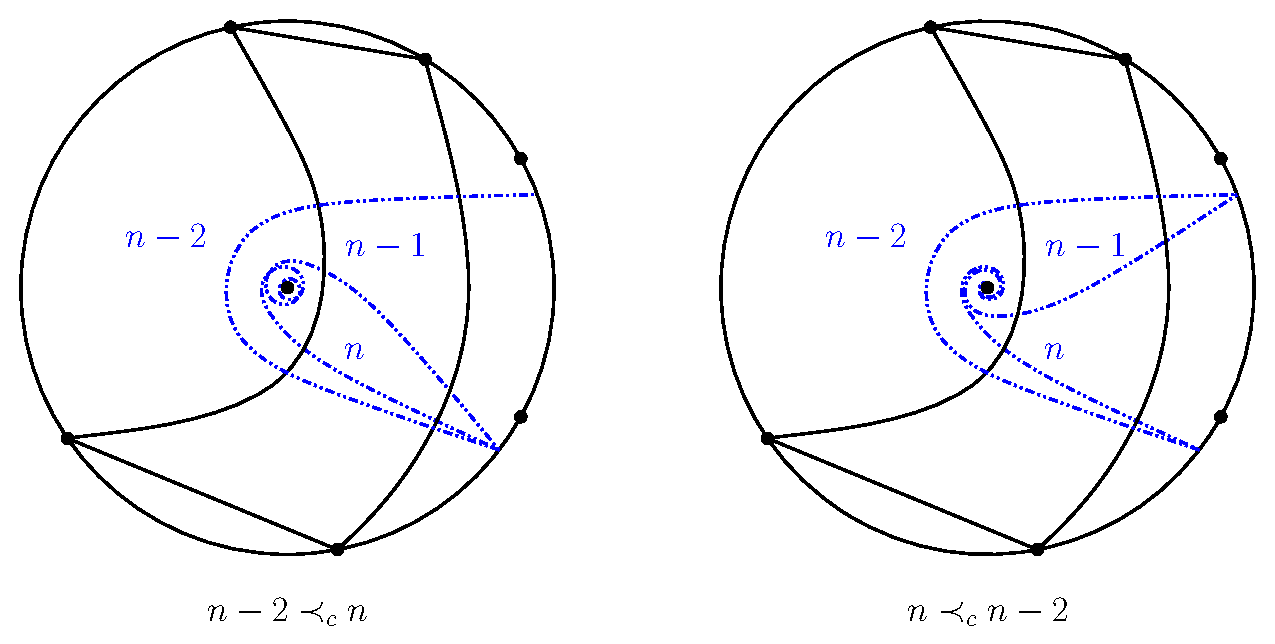
\includegraphics[scale=0.7]{D_n-roots.eps}
    \end{center}
    \caption{Quadrilaterals in type $D_n$ with both diagonals being chords yield unique solutions to \cref{eq:system}.}
    \label{fig:D_n-roots}
  \end{figure}

  \begin{lemma}
    \label{lem:is-radius}
    In all the cases in which \cref{eq:system} is satisfied by two distinct positive roots at least one of $x_\lambda$ and $x_\mu$ corresponds to a radius.
  \end{lemma}
  \begin{proof}
    We will show that, if the arcs corresponding to $x_\lambda$ and $x_\mu$ are both chords, then there is a unique positive root satisfying \cref{eq:system}.
    The two cases to be considered, namely $n-2 \prec_c n$ and  $n \prec_c n-2$, are pictured in \cref{fig:D_n-roots}. 

    Suppose at first that $n-2 \prec_c n$ and let $\alpha$ be one of the two positive roots satisfying \cref{eq:system}.
    By \cref{cor:kernel-Dn}, exactly one among the $(n-1)$-st and the $n$-th simple root coordinates of $\alpha$ is $0$, and the other is $1$.
    In particular, any diagonal of any quadrilateral supporting this exchange relation must give different shear coordinates to the $(n-1)$-st and $n$-th elementary laminations. 
    However, if both diagonals of a quadrilateral are chords, then they do not distinguish the two elementary laminations, so, in particular, each of the two diagonals assigns either $\pm 1$ or $0$ to both simultaneously.

    Suppose now that $n \prec_c n-2$ and let $\alpha$ be again one of the two positive roots satisfying \cref{eq:system}.
    Since one of $\alpha\pm(\alpha_{n-1}+\alpha_n)$ is also a root, the $(n-2)$-nd coordinate of $\alpha$ is $1$ while both the $(n-1)$-st and $n$-th coordinates are simultaneously $1$ or $0$. 
    Thus, any diagonal of any quadrilateral supporting this exchange relation must give shear coordinate $\pm 1$ to the $(n-2)$-nd elementary lamination, and equal values to the $(n-1)$-st and $n$-th ones. 
    Now take any quadrilateral whose diagonals are both chords. 
    If its diagonals give shear coordinate $\pm 1$ to both the $(n-1)$-st and $n$-th elementary lamination, then they assign $\pm 2$ to the $(n-2)$-nd elementary lamination.
    If instead they give shear coordinate $0$ to both $(n-1)$-st and $n$-th elementary laminations, then they also assign $0$ to the $(n-2)$-nd elementary lamination.
  \end{proof}

  \begin{lemma}
    \label{lem:g-vector-of-radii}
    The $\bg$-vector of any cluster variable associated to a radius has exactly one among its $(n-1)$-st and $n$-th fundamental weight coordinates equal to $0$; the other one is $\pm 1$.
  \end{lemma}
  \begin{proof}
    \cite{FST08,FT12} do not contain an explicit recipe to compute the $\bg$-vector of the cluster variable associated to an arc.
    An easy rule, though, can be obtained using \cite[Eq. (1.13)]{NZ12}: it suffices to reflect our surface and compute the shear coordinates of the elementary lamination corresponding to the desired arc with respect to the initial triangulation (see e.g.~\cite[Prop. 5.2]{Re14} or~\cite[Lemma 8.6]{FeTu15}).  
    Since we only care for the last two entries it will suffices to look inside the unique digon in the initial triangulation.
    We are in the situation depicted in \cref{fig:D_n-weights}.
    
    Suppose at first that $n \prec_c n-2$. 
    It follows immediately from \cite[Fig. 36]{FT12} that, in order for a radial elementary lamination to have non-zero $n$-th shear coordinate, it has either to start from the side of the digon lying on the boundary of the disk and then spiral clockwise to the puncture, or cross the other side and spiral counterclockwise. 
    In either case such a lamination will have $(n-1)$-st shear coordinate equal to $0$.
    The situation reverses for radial elementary laminations having non-zero $(n-1)$-st shear coordinate.

    The case $n-2 \prec_c n$ is identical: the two are related by a flip and the only effect this has on the last two shear coordinates is to change some of the signs.
  \end{proof}

  \begin{figure}
    \begin{center}
      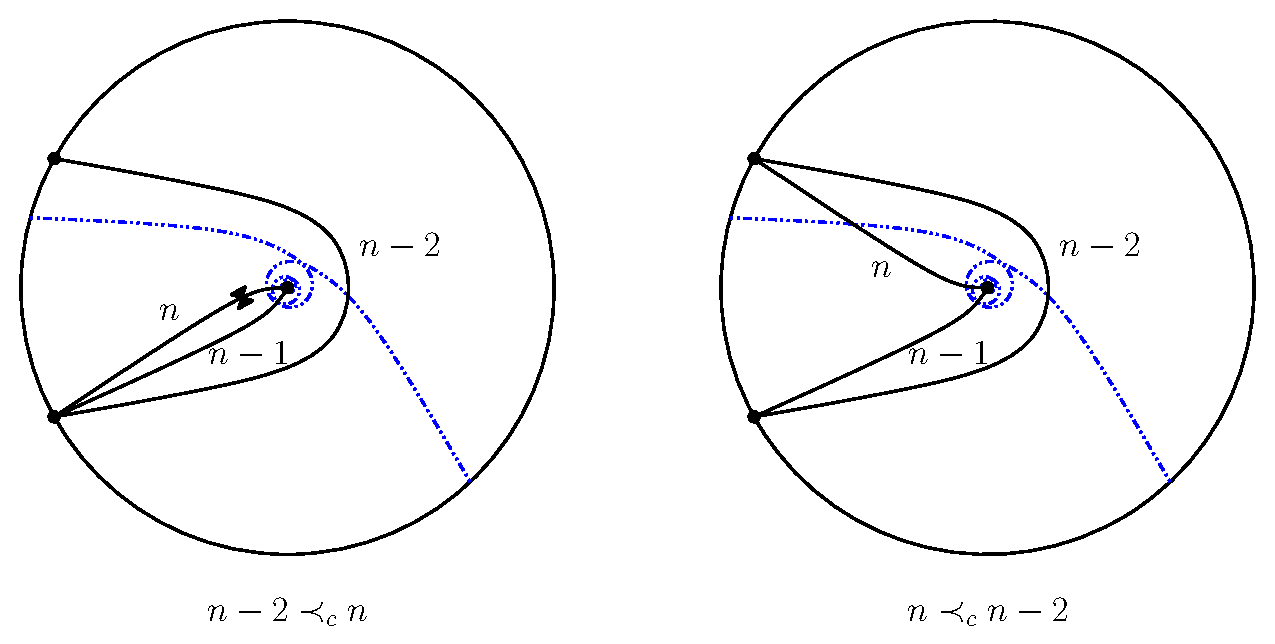
\includegraphics[scale=0.7]{D_n-weights.eps}
    \end{center}
    \caption{Radial laminations with non-zero $n$-th shear coordinate.}
    \label{fig:D_n-weights}
  \end{figure}

  We are finally ready to conclude the proof of \cref{thm:main} in type $D_n$.
  Suppose $\lambda$ and $\mu$ exchangeable weights are such that \cref{eq:system} has two solutions $\alpha$ and $\alpha'$.
  In particular $\alpha' = \alpha \pm (\alpha_{n-1}-\alpha_n)$ if $n-2 \prec_c n$ and $\alpha' = \alpha \pm (\alpha_{n-1}+\alpha_n)$ if $n \prec_c n-2$.
  
  By \cref{lem:is-radius} we can assume that $\lambda$ is the $\bg$-vector of a radius; in particular, by \cref{lem:g-vector-of-radii}
  \[
    \langle \lambda, \alpha_{n-1}\pm \alpha_n \rangle = \pm 1
  \]
  and thus
  \[
    \langle \lambda, \alpha' \rangle =
    \langle \lambda, \alpha \rangle \pm 1.
  \]
  Therefore, since the pairing $\langle\cdot\,,\cdot\rangle$ is integer-valued when computed on (co-)roots and weights, $\alpha$ and $\alpha'$ cannot both satisfy \cref{eq:dual}.

  \begin{remark}
    In view of some ongoing work of the first author with Nathan Reading it appears that a modified version of \cite[Propositions 5.1 and 5.2]{Ste13} holds in affine types as well.
    We expect that \cref{thm:main}, or a refined version of it, could hold there too.
    The analysis required to establish it, though, will probably be more complicated than the finite case one because the corank of $B_c$ can be as big as $4$ and the argument of \cref{rk:induction} does not apply.
  \end{remark}

% bibliography
% HACK: we wanted to have a different label for FeTu15 to distinguish it from FT
% to obtain it from scratch
% 1) uncomment the following two lines
% 2) delete all the pasted text below
% 3) compile file appropriately
% 4) comment again the two lines
% 5) paste the content of finexrel.bbl
% 6) edit as desired

%\bibliographystyle{amsalpha}
%\bibliography{bibliography}

% pasted from finexrel.bbl
\providecommand{\bysame}{\leavevmode\hbox to3em{\hrulefill}\thinspace}
\providecommand{\MR}{\relax\ifhmode\unskip\space\fi MR }
% \MRhref is called by the amsart/book/proc definition of \MR.
\providecommand{\MRhref}[2]{%
  \href{http://www.ams.org/mathscinet-getitem?mr=#1}{#2}
}
\providecommand{\href}[2]{#2}
\begin{thebibliography}{CFZ02}

\bibitem[CFZ02]{CFZ02}
Fr{\'e}d{\'e}ric Chapoton, Sergey Fomin, and Andrei Zelevinsky, \emph{Polytopal
  realizations of generalized associahedra}, Canad. Math. Bull. \textbf{45}
  (2002), no.~4, 537--566, Dedicated to Robert V. Moody. \MR{1941227
  (2003j:52014)}

\bibitem[FST08]{FST08}
Sergey Fomin, Michael Shapiro, and Dylan Thurston, \emph{Cluster algebras and
  triangulated surfaces. {I}. {C}luster complexes}, Acta Math. \textbf{201}
  (2008), no.~1, 83--146. \MR{2448067 (2010b:57032)}

\bibitem[FT12]{FT12}
Sergey Fomin and Dylan Thurston, \emph{{Cluster algebras and triangulated
  surfaces. Part II: Lambda lengths}}, arXiv e-print 1210.5569 (2012).

\bibitem[FeTu15]{FeTu15}
Anna {Felikson} and Pavel {Tumarkin}, \emph{{Bases for cluster algebras from
  orbifolds}}, arXiv e-print 1511.08023 (2015).

\bibitem[FZ02]{FZ02}
Sergey Fomin and Andrei Zelevinsky, \emph{Cluster algebras. {I}.
  {F}oundations}, J. Amer. Math. Soc. \textbf{15} (2002), no.~2, 497--529.
  \MR{1887642}

\bibitem[FZ03]{FZ03}
\bysame, \emph{Cluster algebras. {II}. {F}inite type classification}, Invent.
  Math. \textbf{154} (2003), no.~1, 63--121. \MR{2004457}

\bibitem[FZ07]{FZ07}
\bysame, \emph{Cluster algebras. {IV}. {C}oefficients}, Compos. Math.
  \textbf{143} (2007), no.~1, 112--164. \MR{2295199 (2008d:16049)}

\bibitem[Kac90]{Kac90}
Victor~G. Kac, \emph{Infinite-dimensional {L}ie algebras}, third ed., Cambridge
  University Press, Cambridge, 1990. \MR{1104219 (92k:17038)}

\bibitem[NS14]{NS14}
Tomoki Nakanishi and Salvatore Stella, \emph{Diagrammatic description of
  {$c$}-vectors and {$d$}-vectors of cluster algebras of finite type},
  Electron. J. Combin. \textbf{21} (2014), no.~1, Paper 1.3, 107. \MR{3177498}

\bibitem[NZ12]{NZ12}
Tomoki Nakanishi and Andrei Zelevinsky, \emph{On tropical dualities in cluster
  algebras}, Algebraic groups and quantum groups, Contemp. Math., vol. 565,
  Amer. Math. Soc., Providence, RI, 2012, pp.~217--226. \MR{2932428}

\bibitem[Rea14]{Re14}
Nathan Reading, \emph{Universal geometric cluster algebras from surfaces},
  Trans. Amer. Math. Soc. \textbf{366} (2014), no.~12, 6647--6685. \MR{3267022}

\bibitem[Ste13]{Ste13}
Salvatore Stella, \emph{Polyhedral models for generalized associahedra via
  {C}oxeter elements}, J. Algebraic Combin. \textbf{38} (2013), no.~1,
  121--158. \MR{3070123}

\bibitem[YZ08]{YZ08}
Shih-Wei Yang and Andrei Zelevinsky, \emph{Cluster algebras of finite type via
  {C}oxeter elements and principal minors}, Transform. Groups \textbf{13}
  (2008), no.~3-4, 855--895. \MR{2452619 (2009j:13029)}

\end{thebibliography}
% end pasted from finextel.bbl

\end{document}
